% !TEX root = ../beamer.tex

\begin{frame}
    \frametitle{Our Procedure}
    \begin{itemize}
   \item Agile software development using the Scrum methodology
   \item Scrum board with user stories and responsibilities
    \end{itemize}
    \vfill
    \begin{center}
		\begin{tikzpicture}
			\node[fill=white, draw, drop shadow] {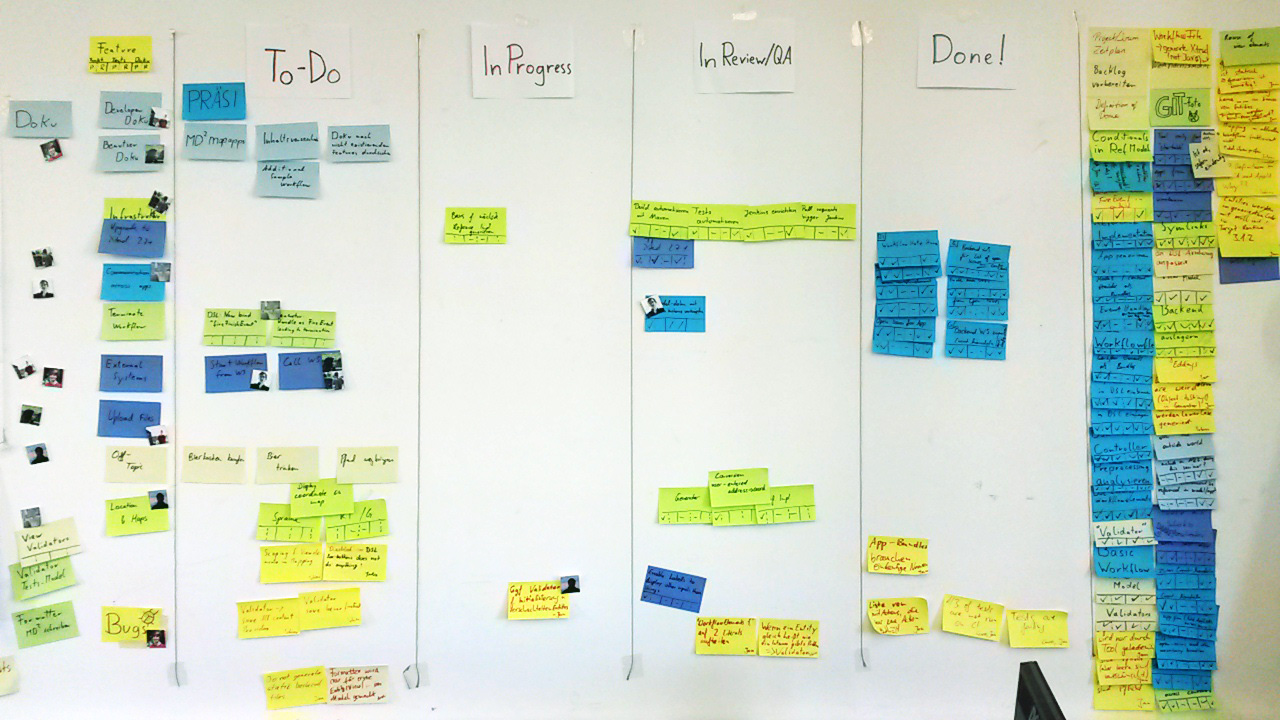
\includegraphics[height=40mm]{images/scrumboard}};
		\end{tikzpicture}
    \end{center}
\end{frame}

%-----------------------------------------------------------------------------------

\begin{frame}
\frametitle{Story Cards}
\begin{center}
	\begin{tikzpicture}[
		line/.style= {pantone396!50!black},
		lbl/.style= {}
	]
		\draw[fill=pantone396!10!white, draw=pantone396] (0,0) rectangle (9, 6);
		\draw[line] (0, 2) -- (9, 2);
		\foreach \x in {1.5, 4.5, 7.5}
			\draw[line, dashed] (\x, 0) -- (\x, 2);
		\foreach \x in {3, 6}
			\draw[line, ] (\x, 0) -- (\x, 2);
		
		\node[lbl] at (1.5, 2.25) {\scriptsize{Implementation\vphantom{Aq}}};
		\node[lbl] at (4.5, 2.25) {\scriptsize{Tests\vphantom{Aq}}};
		\node[lbl] at (7.5, 2.25) {\scriptsize{Documentation\vphantom{Aq}}};
		
		\node[] at (4.5, 4) {\Large{Task Description}};
		
		\node at (0.75, 1.1) {\LARGE{\textbf{\checkmark}}};
		\node at (3.75, 1.1) {\LARGE{\textbf{\checkmark}}};
		
		\foreach \x in {0.75, 3.75, 6.75}
			\node at (\x, 0.2) {\tiny{DONE}};
		\foreach \x in {2.25, 5.25, 8.25}
			\node at (\x, 0.2) {\tiny{REVIEWED}};
			
		\node[overlay, inner sep = 0, draw, rotate=6] at (7.5, 5.75) {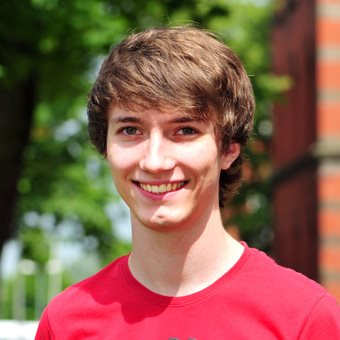
\includegraphics[width=1.75cm]{images/malte}};
		
	\end{tikzpicture}
\end{center}
\end{frame}

%-----------------------------------------------------------------------------------

%\begin{frame}
%    \frametitle{Scrum} 
%    \begin{center}
%		\begin{tikzpicture}
%			\node[fill=white, draw, drop shadow] {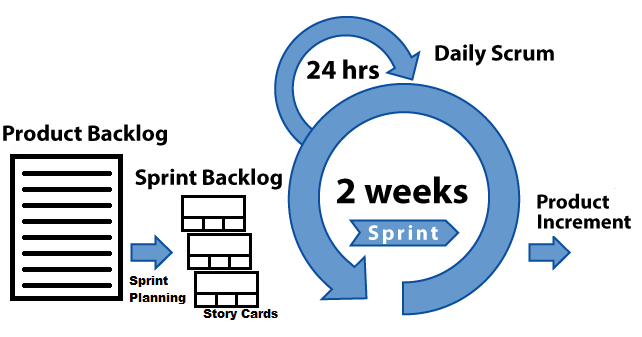
\includegraphics[height=40mm]{images/scrum-overview.png}};
%		\end{tikzpicture}
%    \end{center}
%\end{frame}

%-----------------------------------------------------------------------------------

%\begin{frame}
%   \frametitle{Scrum Board}
%       \begin{center}   
%   	    \begin{tikzpicture}
%   	       \draw[-, lightgray] (0,0) -- (10,0);
%   	       
%   	       \draw[-, lightgray] (2,0.5) -- (2,-3);
%   	       \node [above] at (1,0) {\small{\textbf{User Story\vphantom{Aq}}}};
%   	       \node [above] at (1,-1) {\small{Story 1}};
%   	       \node [above] at (1,-1.3) {\tiny{responsible: Malte\vphantom{Aq}}};
%   	       \node [above] at (1,-2) {\small{Story 2}};
%   	       \node [above] at (1,-2.3) {\tiny{responsible: Jan\vphantom{Aq}}};
%   	       
%   	       \draw[-, lightgray] (4,0.5) -- (4,-3);
%   	       \node [above] at (3,0) {\small{\textbf{Todo\vphantom{Aq}}}};
%   	       \node [above] at (3,-1) {\small{Story Cards\vphantom{Aq}}};
%   	       \node [above] at (3,-1.3) {\tiny{Card1, Card2, ...}\vphantom{Aq}};
%   	       \node [above] at (3,-2) {\small{Story Cards\vphantom{Aq}}};
%   	       \node [above] at (3,-2.3) {\tiny{Card1, Card2, ...\vphantom{Aq}}};
%   	       
%   	       \draw[-, lightgray] (6,0.5) -- (6,-3);
%   	       \node [above] at (5,0) {\small{\textbf{In Progress\vphantom{Aq}}}};
%   	       \node [above] at (5,-1) {\small{Card3\vphantom{Aq}}};
%   	       
%   	       \draw[-, lightgray] (8,0.5) -- (8,-3);
%   	       \node [above] at (7,0) {\small{\textbf{In Review\vphantom{Aq}}}};
%   	       \node [above] at (7,-2) {\small{Card4\vphantom{Aq}}};
%   	       
%   	       \node [above] at (9,0) {\small{\textbf{Done\vphantom{Aq}}}};
%   	       \node [above] at (9,-1) {\small{Card5\vphantom{Aq}}};
%   	       \node [above] at (9,-2) {\small{Card6\vphantom{Aq}}};
%   	       
%   	    \end{tikzpicture}
%   	   \end{center}
%\end{frame}

%-----------------------------------------------------------------------------------

\begin{frame}
	\frametitle{Our Scrum Board}
    \begin{figure}
	    \begin{center}
	        \pgfimage[height=60mm]{images/scrum.png}
	    \end{center}
	\end{figure}
\end{frame}

%-----------------------------------------------------------------------------------

\begin{frame}[plain]
	\frametitle{User Stories Over Time}
	\begin{center}
		\begin{tikzpicture}[
			>=stealth,x=.08cm,y=.15cm,
			lbl/.style = {minimum height = 1cm},
			lbl1/.style = {lbl, anchor = east},
			lbl2/.style = {lbl, anchor = west},
			box/.style = {draw=pantone315, fill=pantone315!50!white}		
		]
			\draw[dotted] (-15, -1) -- ++(5, 0);
			\draw[->] (-10, -1) -- ++(125, 0);
			\draw (4,-1) -- ++(0,-4pt) node [below] {Dec};
			\draw (35,-1) -- ++(0,-4pt) node [below] {Jan};
			\draw (66,-1) -- ++(0,-4pt) node [below] {Feb};
			\draw (94,-1) -- ++(0,-4pt) node [below] {Mar};
			
			\draw[box]  (79, 1) rectangle (111, 3); \node[lbl1] at (79, 2) {\scriptsize{}Documentation and presentation};
			\draw[box]  (79, 4) rectangle (111, 6); \node[lbl1] at (79, 5) {\scriptsize{}External systems};
			\draw[box]  (79, 7) rectangle (111, 9); \node[lbl1] at (79, 8) {\scriptsize{}File upload};
			
			\draw[box] (79, 10) rectangle (96, 12); \node[lbl1] at (79, 11) {\scriptsize{}Terminate workflow};
			\draw[box] (79, 13) rectangle (96, 15); \node[lbl1] at (79, 14) {\scriptsize{}Upgrade to Xtext 2.7.1};
			
			\draw[box] (67, 16) rectangle (96, 18); \node[lbl1] at (67, 17) {\scriptsize{}Location \& maps};
			\draw[box] (50, 19) rectangle (88, 21); \node[lbl1] at (50, 20) {\scriptsize{}Communication across apps};
			
			\draw[box] (41, 22) rectangle (67, 24); \node[lbl1] at (41, 23) {\scriptsize{}Reuse of view elements};
			\draw[box] (41, 25) rectangle (67, 27); \node[lbl1] at (41, 26) {\scriptsize{}Workflow};
			\draw[box] (41, 28) rectangle (50, 30); \node[lbl1] at (41, 29) {\scriptsize{}Communication with outside world};
			
			\draw[box] (15, 31) rectangle (96, 33); \node[lbl1] at (15, 32) {\scriptsize{}Infrastructure}; % infrastructure
			
			\draw[box] (1, 34) rectangle (50, 36); \node[lbl2] at (50, 35) {\scriptsize{}DSL tests (legacy)}; %DSL tests legacy
			\draw[box] (1, 37) rectangle (41, 39); \node[lbl2] at (41, 38) {\scriptsize{}Basic workflow}; % basic workflow
			\draw[box] (1, 40) rectangle (15, 42); \node[lbl2] at (15, 41) {\scriptsize{}Conditionals in reference model}; % conditionals			
			
		\end{tikzpicture}	
	\end{center}
\end{frame}

%-----------------------------------------------------------------------------------

\begin{frame}[plain]
	\frametitle{Bugs}
	\plainnumber
    \begin{center}
		\begin{tikzpicture}
			\node[fill=white, draw, drop shadow] {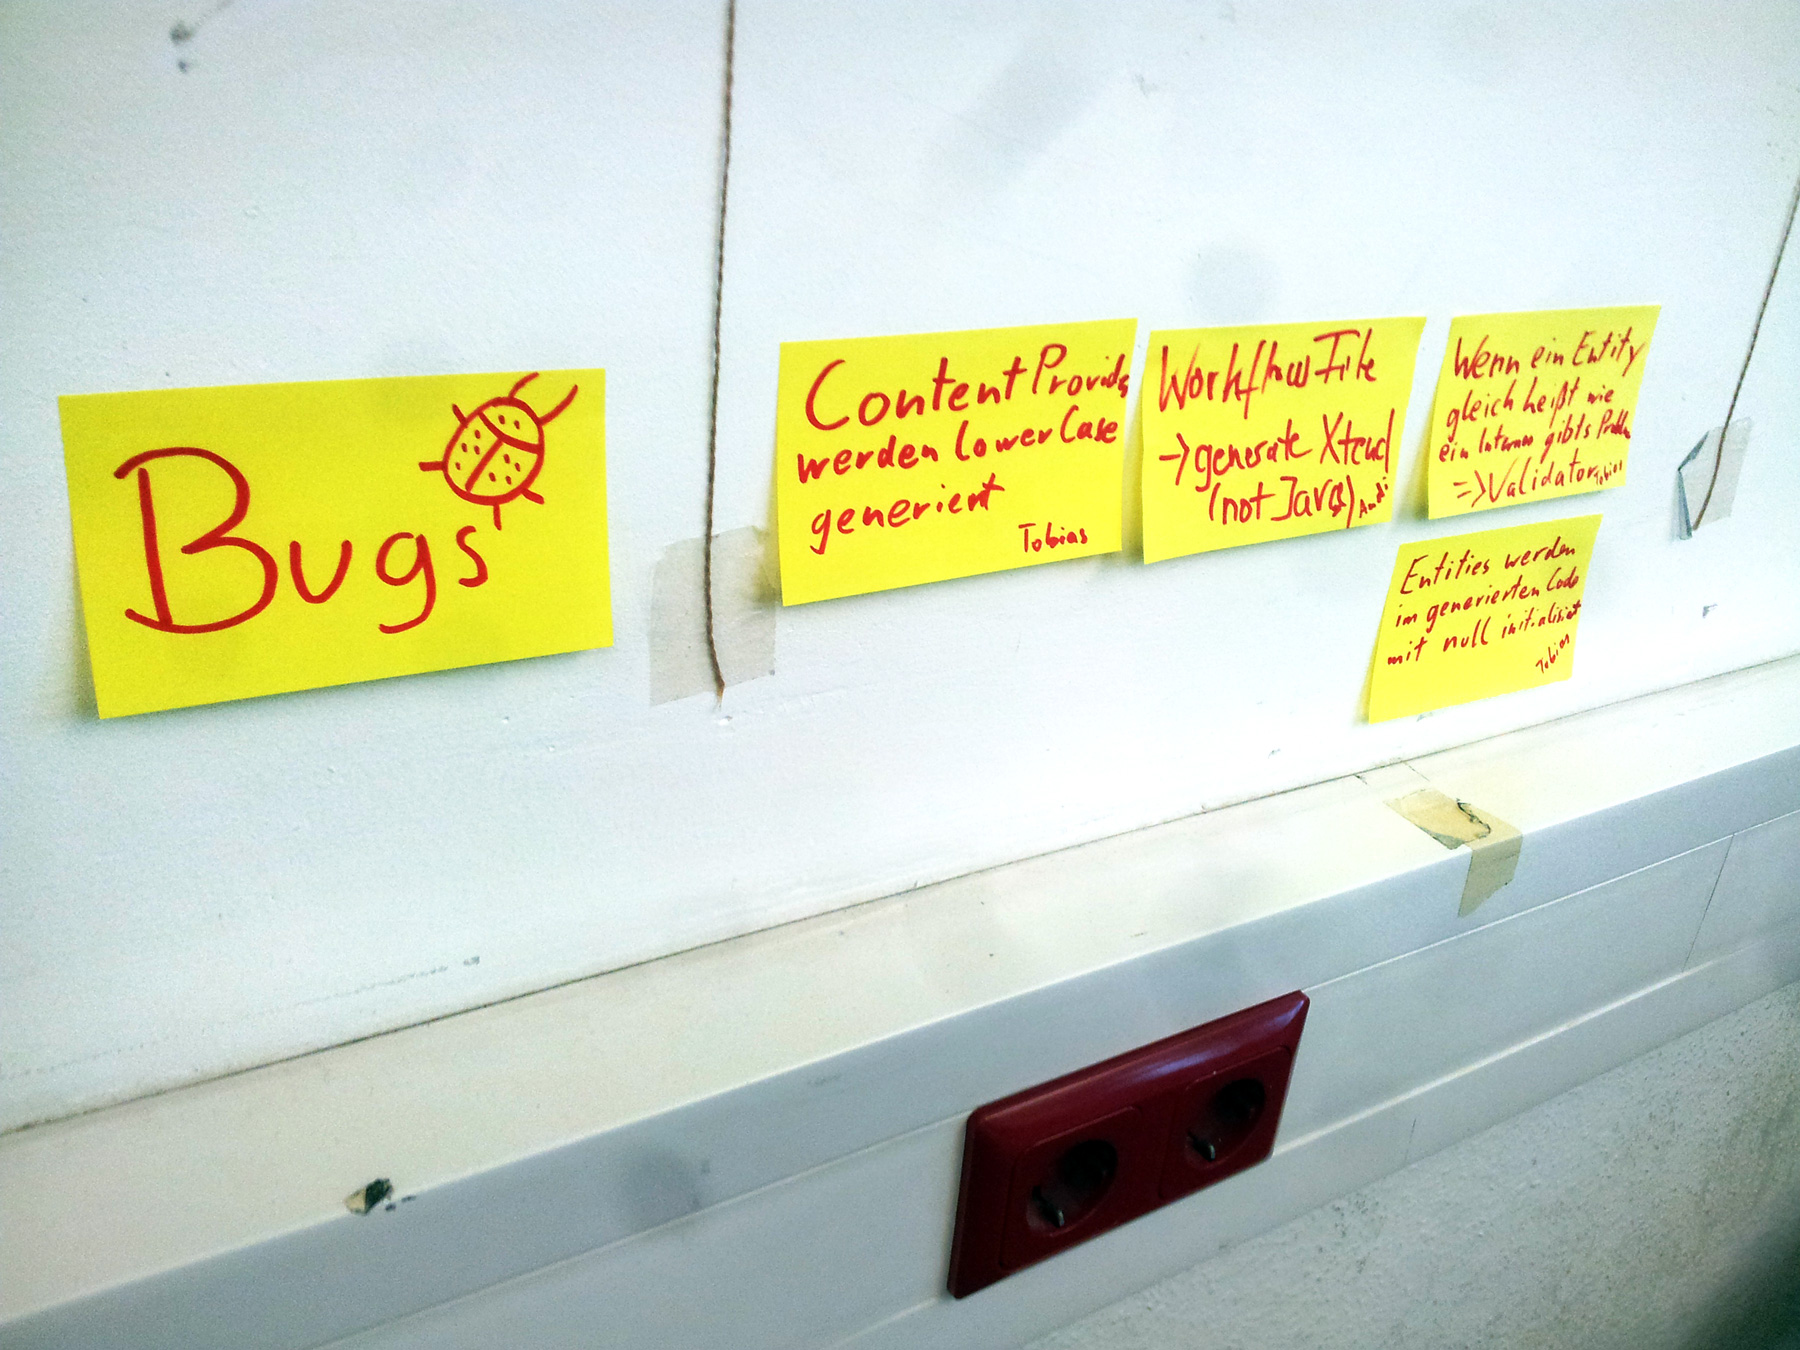
\includegraphics[width=.85\textwidth]{images/bugs}};
		\end{tikzpicture}
    \end{center}
\end{frame}

%-----------------------------------------------------------------------------------

\begin{frame}[fragile]
    \frametitle{Bug Fixes}

\begin{itemize}
  \item Disable a button \tiny{(e.g., "Previous" button in first view)}  
\end{itemize}

\begin{center}
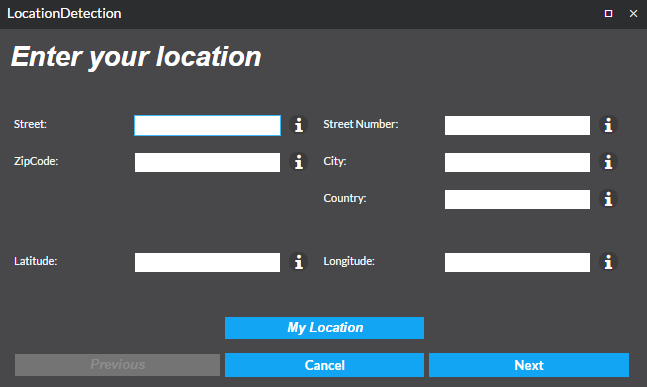
\includegraphics[width=0.6\textwidth] {images/disabled-previous-button.png}
\end{center}

\vspace{-1ex}

\begin{lstlisting}[basicstyle=\footnotesize\ttfamily]
Button MyPreviousBtn { 
  style button text "Previous" disabled true
}
\end{lstlisting}

\end{frame}	

%-----------------------------------------------------------------------------------

\begin{frame}
    \frametitle{Continuous Integration with Jenkins}
    
    \begin{figure}
    	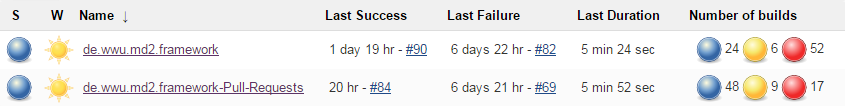
\includegraphics[width= 0.9\linewidth]{images/jenkins-jobs.png}
    \end{figure}
    
    \vspace{-1ex}
    
    \begin{itemize}
       \item \texttt{de.wwu.md2.framework}
       \begin{itemize}
           \item builds every time the \texttt{mapapps} branch is updated
       \end{itemize}
       \item \texttt{de.wwu.md2.framework-Pull-Requests} 
       \begin{itemize}
           \item builds for each pull request
           \item merged with current \texttt{mapapps} branch
       \end{itemize}
    \end{itemize}
\end{frame}

%-----------------------------------------------------------------------------------

\begin{frame}[plain]
\frametitle{Test Trend Chart: \texttt{mapapps} branch}
\plainnumber
\begin{center}
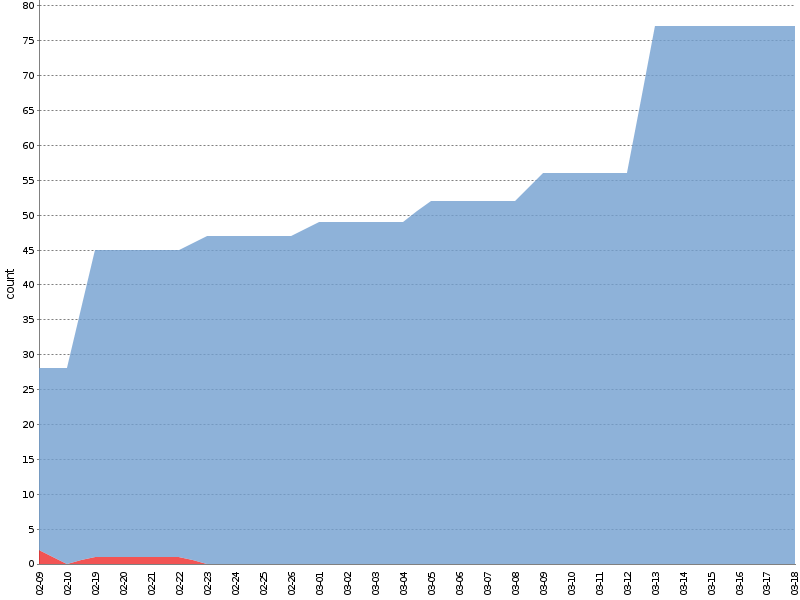
\includegraphics[width=1\textwidth] {images/test-trend-chart-md2-framework.png}
\end{center}
\end{frame}

%-----------------------------------------------------------------------------------

\begin{frame}[fragile]
\frametitle{Testing the validator of a WS call}

\begin{lstlisting}
externalWebService sendEmail { 
  url "http://psmd2.uni-muenster.de:8080/SendMail/api/mail/send/" 
  method GET 
  queryparams ( 
    "to" : "andreas.fuchs@uni-muenster.de" 
    "subject" : "The Subject" 
    "body" : "Hello Andreas, this is the message for you."
  )
  bodyparams(
    "test" : "test"
  )
}
\end{lstlisting}
\end{frame}

\begin{frame}[fragile]
\frametitle{Testing the validator of a WS call}

\codeheading{Test implementation}
\begin{lstlisting}
@Test
def noBodyParamsAllowedWhenGETMethodTest(){
    ws_call_validator_model.assertError(
        MD2Package::eINSTANCE.webServiceCall,
        ControllerValidator::NOBODYPARAMSWHENGET);
}
\end{lstlisting}

\vfill

\codeheading{Validator implementation}
\begin{lstlisting}
@Check
def checkNoBodyParamsWhenGETMethod(WebServiceCall wscall){
    if(wscall.method.equals(RESTMethod.GET) 
       && wscall.bodyparams.size > 0) {
        acceptError("...");
    }
}
\end{lstlisting}

\end{frame}

%-----------------------------------------------------------------------------------

%\begin{frame}[plain]
%\frametitle{Test Trend Chart: pull requests}
%\plainnumber
%\begin{center}
%\includegraphics[width=1\textwidth, clip = true] %{images/test-trend-chart-md2-pull-requests.png}
%\end{center}
%\end{frame}

%-----------------------------------------------------------------------------------



